\documentclass[tikz,border=10pt]{standalone}
\usepackage{tikz}
\usetikzlibrary{arrows.meta,positioning}

\tikzset{
  card/.style={draw=blue!70!black, line width=1.2pt, rounded corners=3pt, minimum width=3.2cm, minimum height=1.0cm, align=center, fill=none},
  result/.style={draw=orange!80!black, line width=1.2pt, rounded corners=3pt, minimum width=3.6cm, minimum height=1.0cm, align=center, fill=none},
  flow/.style={-{Stealth[length=3mm]}, line width=1.2pt, draw=black!70}
}

\begin{document}
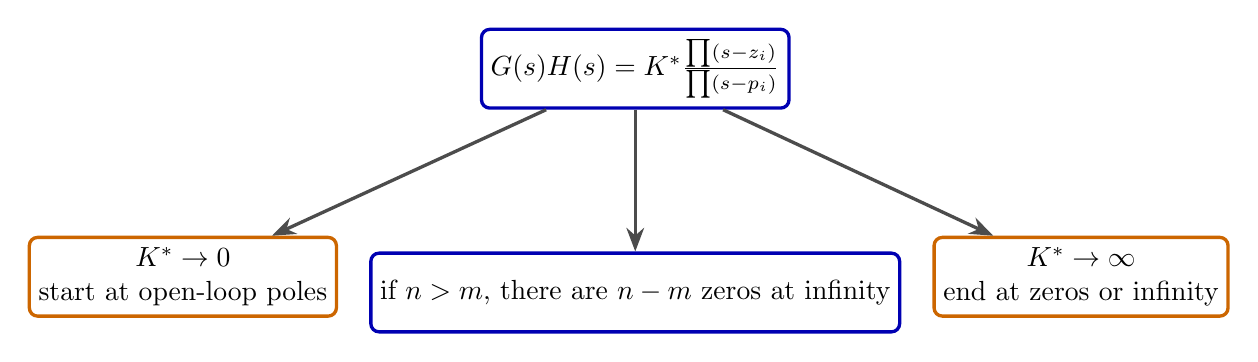
\begin{tikzpicture}[node distance=0.9cm and 1.0cm]
  \node[card] (eq) {$G(s)H(s)=K^\ast \frac{\prod(s-z_i)}{\prod(s-p_i)}$};
  \node[result, below left=1.6cm and 1.8cm of eq] (start) {$K^\ast \to 0$\\start at open-loop poles};
  \node[result, below right=1.6cm and 1.8cm of eq] (end) {$K^\ast \to \infty$\\end at zeros or infinity};
  \node[card, below=1.8cm of eq] (infz) {if $n>m$, there are $n-m$ zeros at infinity};

  \draw[flow] (eq) -- (start);
  \draw[flow] (eq) -- (end);
  \draw[flow] (eq) -- (infz);
\end{tikzpicture}
\end{document}
